\documentclass[11pt,a4paper,fontset=fandol]{ctexart}

% ====== 版面 ======
\usepackage{geometry}
\geometry{a4paper, left=2.2cm, right=2.2cm, top=2.2cm, bottom=2.2cm, headheight=14pt}
\usepackage{setspace}
\linespread{1.05}
\usepackage{indentfirst}
\setlength{\parindent}{2em}
\emergencystretch=2em

% ====== 颜色 ======
\usepackage{xcolor}
\definecolor{themecolor}{RGB}{40,90,140}
\definecolor{codebg}{RGB}{248,248,245}

% ====== 图、表、数学 ======
\usepackage{graphicx}
\graphicspath{{results/}}
\usepackage{amsmath}
\usepackage{booktabs}
\usepackage{caption}
\captionsetup{font=small,labelfont={bf,color=themecolor}}
\usepackage{subcaption}
\usepackage{float}
\usepackage{array}
\usepackage{verbatim}

% ====== 链接 ======
\usepackage{hyperref}
\hypersetup{
  colorlinks=true,
  linkcolor=themecolor,
  citecolor=themecolor,
  urlcolor=themecolor!70!black,
}

% ====== 章节样式：主题色 + 横线分割 ======
\usepackage{titlesec}
\titleformat{\section}
  {\color{themecolor}\bfseries\fontsize{13}{16}\selectfont}
  {\thesection}{0.6em}{}
\titlespacing*{\section}{0pt}{0.9em}{0.35em}

\titleformat{\subsection}
  {\color{themecolor!85!black}\bfseries\fontsize{11.5}{14}\selectfont}
  {\thesubsection}{0.6em}{}
\titlespacing*{\subsection}{0pt}{0.55em}{0.15em}

% ====== 页眉页脚 ======
\usepackage{fancyhdr}
\pagestyle{fancy}
\fancyhf{}
\renewcommand{\headrulewidth}{0.4pt}
\lhead{\small\color{black!55} 键控机器人运动实验报告}
\rhead{\small\color{black!55} 人工智能 2302}
\cfoot{\small\color{black!55}\thepage}

\fancypagestyle{plain}{
  \fancyhf{}
  \renewcommand{\headrulewidth}{0pt}
  \cfoot{\small\color{black!55}\thepage}
}

% ====== 代码块加浅色边框 ======
\usepackage{mdframed}
\BeforeBeginEnvironment{verbatim}{
  \begin{mdframed}[
    backgroundcolor=codebg,
    linecolor=themecolor!30,
    linewidth=0.5pt,
    innerleftmargin=10pt,
    innerrightmargin=8pt,
    innertopmargin=6pt,
    innerbottommargin=4pt,
    skipabove=8pt,
    skipbelow=8pt,
    roundcorner=2pt,
  ]
}
\AfterEndEnvironment{verbatim}{\end{mdframed}}

\setCJKmonofont{Arial Unicode MS}

% ====== 标题页信息 ======
\title{\bfseries 键控机器人运动实验报告}
\author{人工智能2302 \quad 蒋梓轩\\
人工智能2302 \quad 汪翌秦\\
人工智能2302 \quad 孙靖淞}
\date{2026 年 5 月 21 日}

\begin{document}

\maketitle

\section{实验目的}

本次实验围绕 ROS 机器人模型可视化、TF 坐标变换和键盘遥控展开。实验首先部署 ROS Noetic 环境和小车运行环境，再通过 URDF/Xacro 文件描述小车连杆和关节结构，在 RViz 中加载机器人模型并观察 TF 树；随后补全仿真节点，使其订阅键盘控制节点发布的 \verb|/cmd_vel| 速度指令，并发布 \verb|/odom| 里程计信息和 \verb|odom -> base_footprint| 坐标变换；最后在实体小车上完成底盘启动、悬空安全测试和落地遥控运动。

通过本次实验，需要掌握三个重点：第一，理解 URDF 中 \verb|robot|、\verb|link|、\verb|joint| 标签如何抽象小车结构；第二，理解 TF 树中各坐标系的父子关系，尤其是 \verb|odom| 与 \verb|base_footprint| 的动态关系；第三，理解 \verb|/cmd_vel| 是控制命令，\verb|/odom| 是状态反馈，两者共同构成机器人运动控制中的输入与观测链路。

\section{实验原理}

URDF 文件本质上是一个描述机器人结构的 XML 文件，\verb|link| 表示机器人上的刚体部件，\verb|joint| 表示两个部件之间的连接关系。RViz 不负责物理仿真，它主要用于可视化 ROS 消息和坐标系关系，因此需要先把 URDF 载入参数服务器中的 \verb|robot_description|，再由 \verb|robot_state_publisher| 根据关节状态发布各个 link 之间的 TF。

键控运动部分使用 \verb|teleop_twist_keyboard| 节点。该节点读取键盘按键，把线速度和角速度封装成 \verb|geometry_msgs/Twist| 消息后发布到 \verb|/cmd_vel|。仿真或实车底盘节点订阅该话题，根据速度命令更新机器人状态；同时发布 \verb|nav_msgs/Odometry| 类型的 \verb|/odom| 话题，并通过 TF 广播 \verb|odom| 到机器人底盘坐标系的变换。

\begin{table}[H]
  \centering
  \caption{本实验中的关键 ROS 话题与作用}
  \begin{tabular}{llll}
    \toprule
    话题 & 消息类型 & 典型发布方 & 典型订阅方 \\
    \midrule
    \verb|/cmd_vel| & \verb|geometry_msgs/Twist| & 键盘遥控节点 & 仿真节点/底盘驱动 \\
    \verb|/odom| & \verb|nav_msgs/Odometry| & 仿真节点/底盘驱动 & RViz、导航模块 \\
    \verb|/tf| & \verb|tf2_msgs/TFMessage| & 状态发布节点/底盘节点 & RViz、TF 工具 \\
    \verb|/joint_states| & \verb|sensor_msgs/JointState| & 关节状态发布节点 & 机器人状态发布节点 \\
    \bottomrule
  \end{tabular}
  \label{tab:topics}
\end{table}

\section{实验步骤与结果分析}

\subsection{ROS 环境与代码配置}

按照指导书要求，实验环境使用 Ubuntu 20.04 与 ROS Noetic。仿真端创建 \verb|catkin_ebot_sim| 工作空间和 \verb|vehicle_sim| 功能包，依赖项包括 \verb|rospy|、\verb|geometry_msgs|、\verb|nav_msgs|、\verb|tf2_ros|、\verb|urdf| 和 \verb|xacro|；实车端在小车系统中启动 ROS Noetic Docker 容器，确认 \verb|teleop_twist_keyboard| 可用，并通过底盘启动 launch 文件连接小车驱动。

根据“完善 \verb|vehicle_sim.py|”的要求，仿真节点完成三件事：订阅 \verb|/cmd_vel|，将线速度和角速度按时间积分为 $x$、$y$、$\theta$；发布 \verb|nav_msgs/Odometry| 类型的 \verb|/odom|；使用 \verb|tf2_ros.TransformBroadcaster| 广播 \verb|odom| 到 \verb|base_footprint| 的动态坐标变换。launch 文件同时启动 RViz、关节状态发布节点、机器人状态发布节点和 \verb|vehicle_sim_node|。

\subsection{仿真模型加载与 TF 可视化}

RViz 启动后，将 Fixed Frame 设置为 \verb|base_footprint| 或 \verb|odom|，并添加 RobotModel 与 TF 显示项。从图 \ref{fig:rviz-tf} 可以看到，小车模型已经正确加载，RobotModel 与 TF 均处于启用状态；通过 rqt\_tf\_tree 或 TF 显示项可以看到车体坐标系、前后轮坐标系等通过树状结构连接在一起，满足 TF 树唯一父节点、无环和连通性要求。

\begin{figure}[H]
  \centering
  \begin{subfigure}{0.49\linewidth}
    \centering
    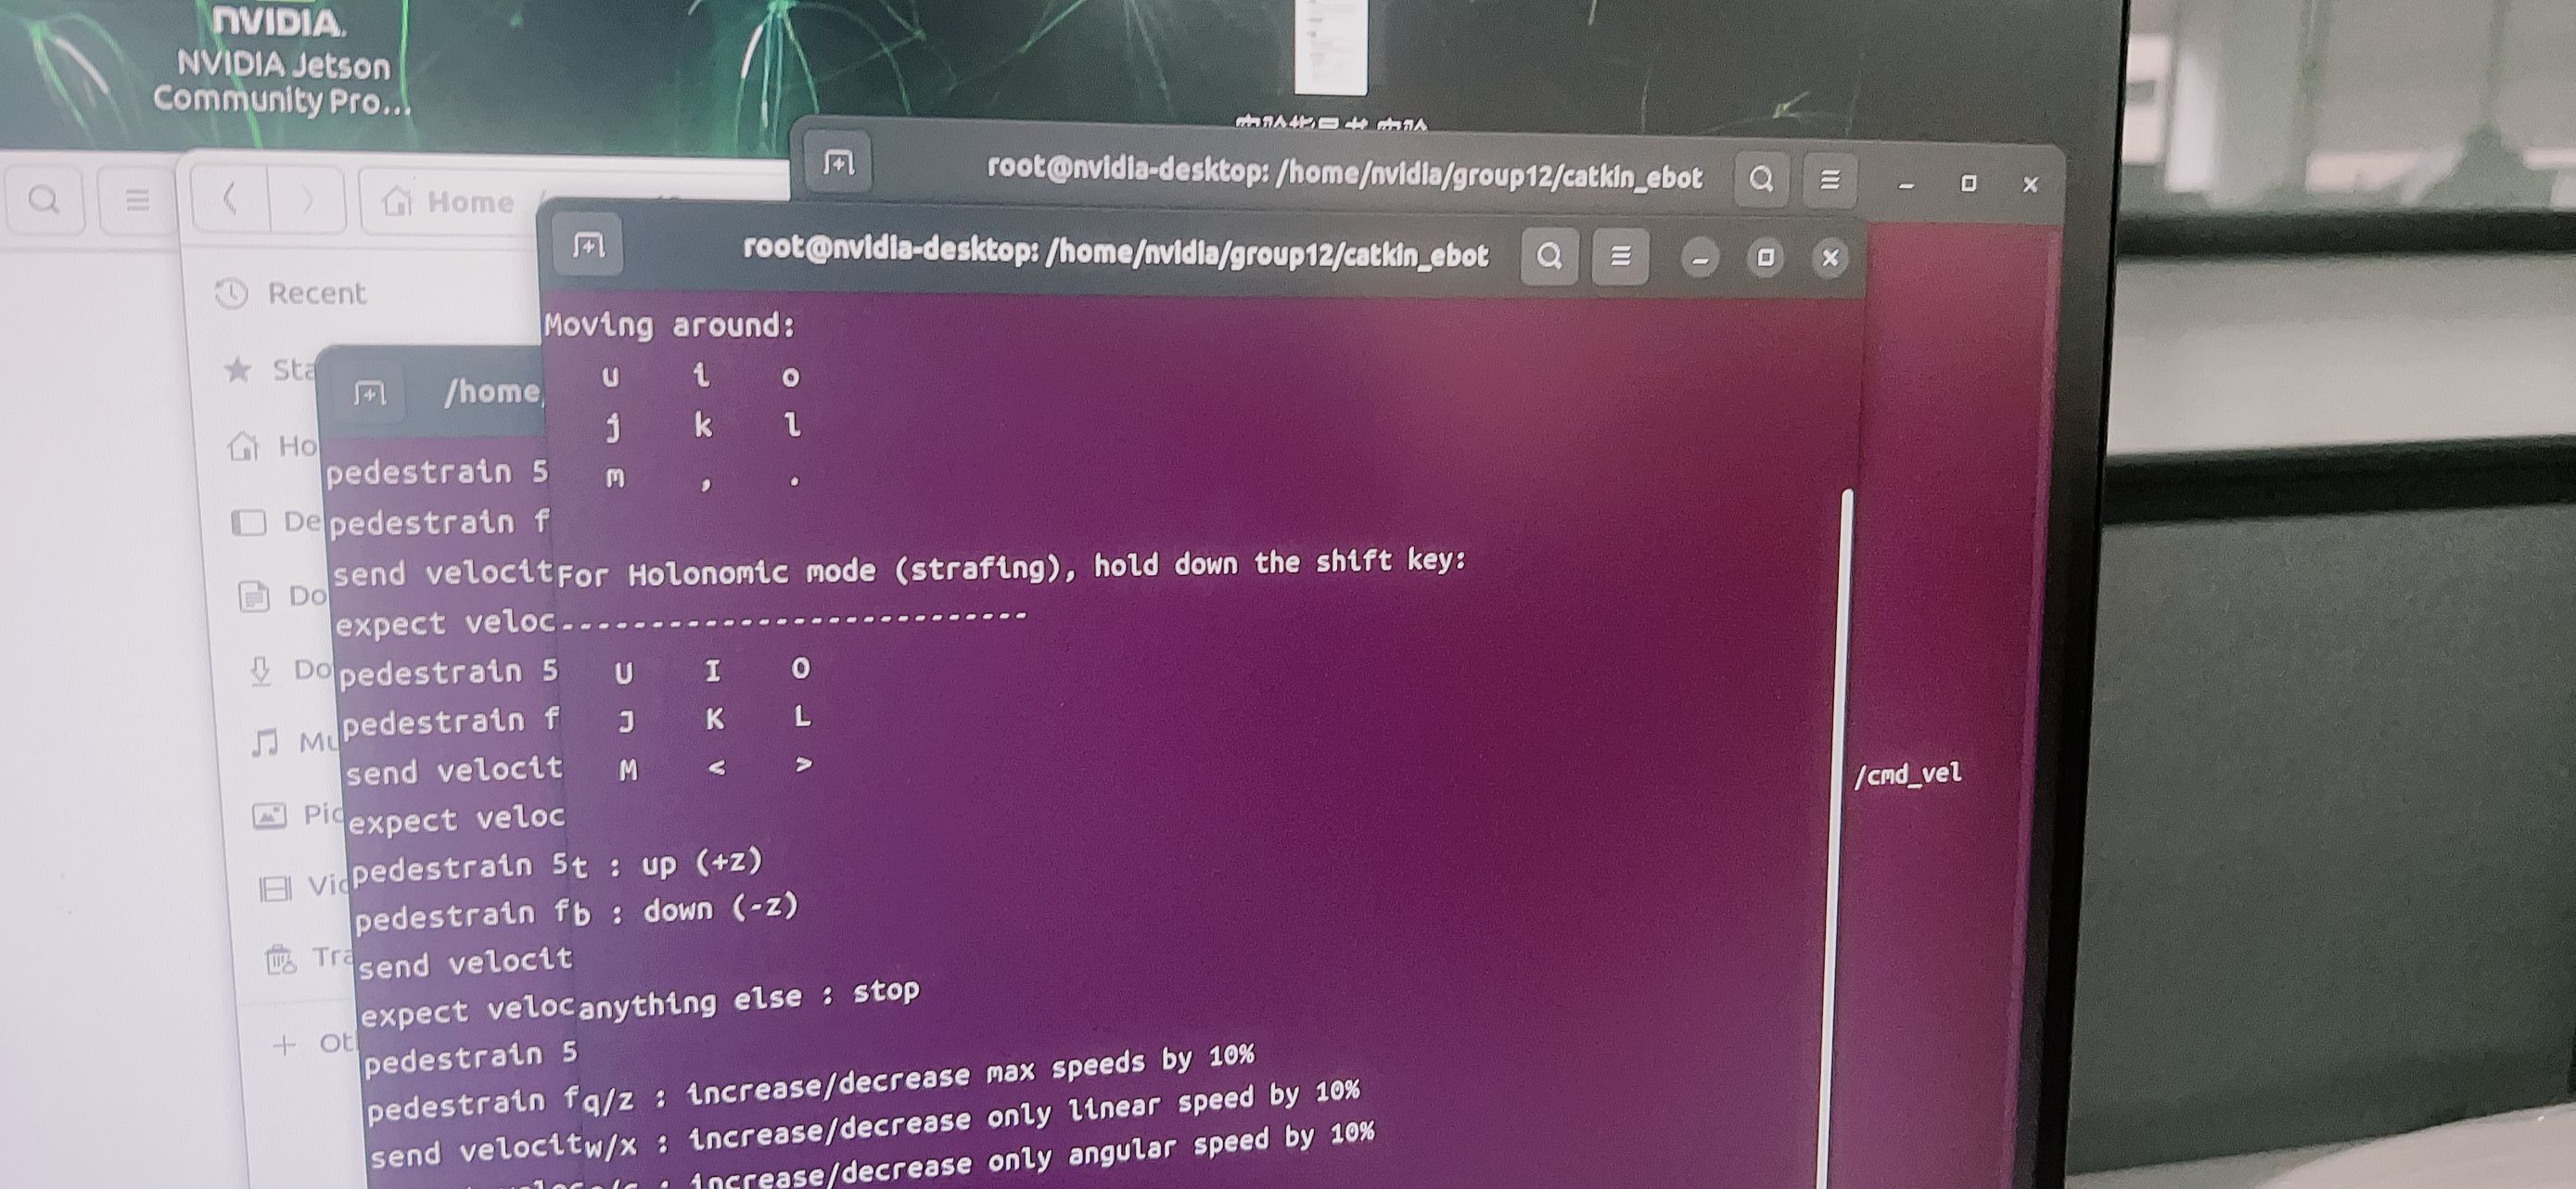
\includegraphics[width=\linewidth]{rviz_model.png}
    \caption{RViz 中加载小车模型与 TF}
  \end{subfigure}
  \hfill
  \begin{subfigure}{0.49\linewidth}
    \centering
    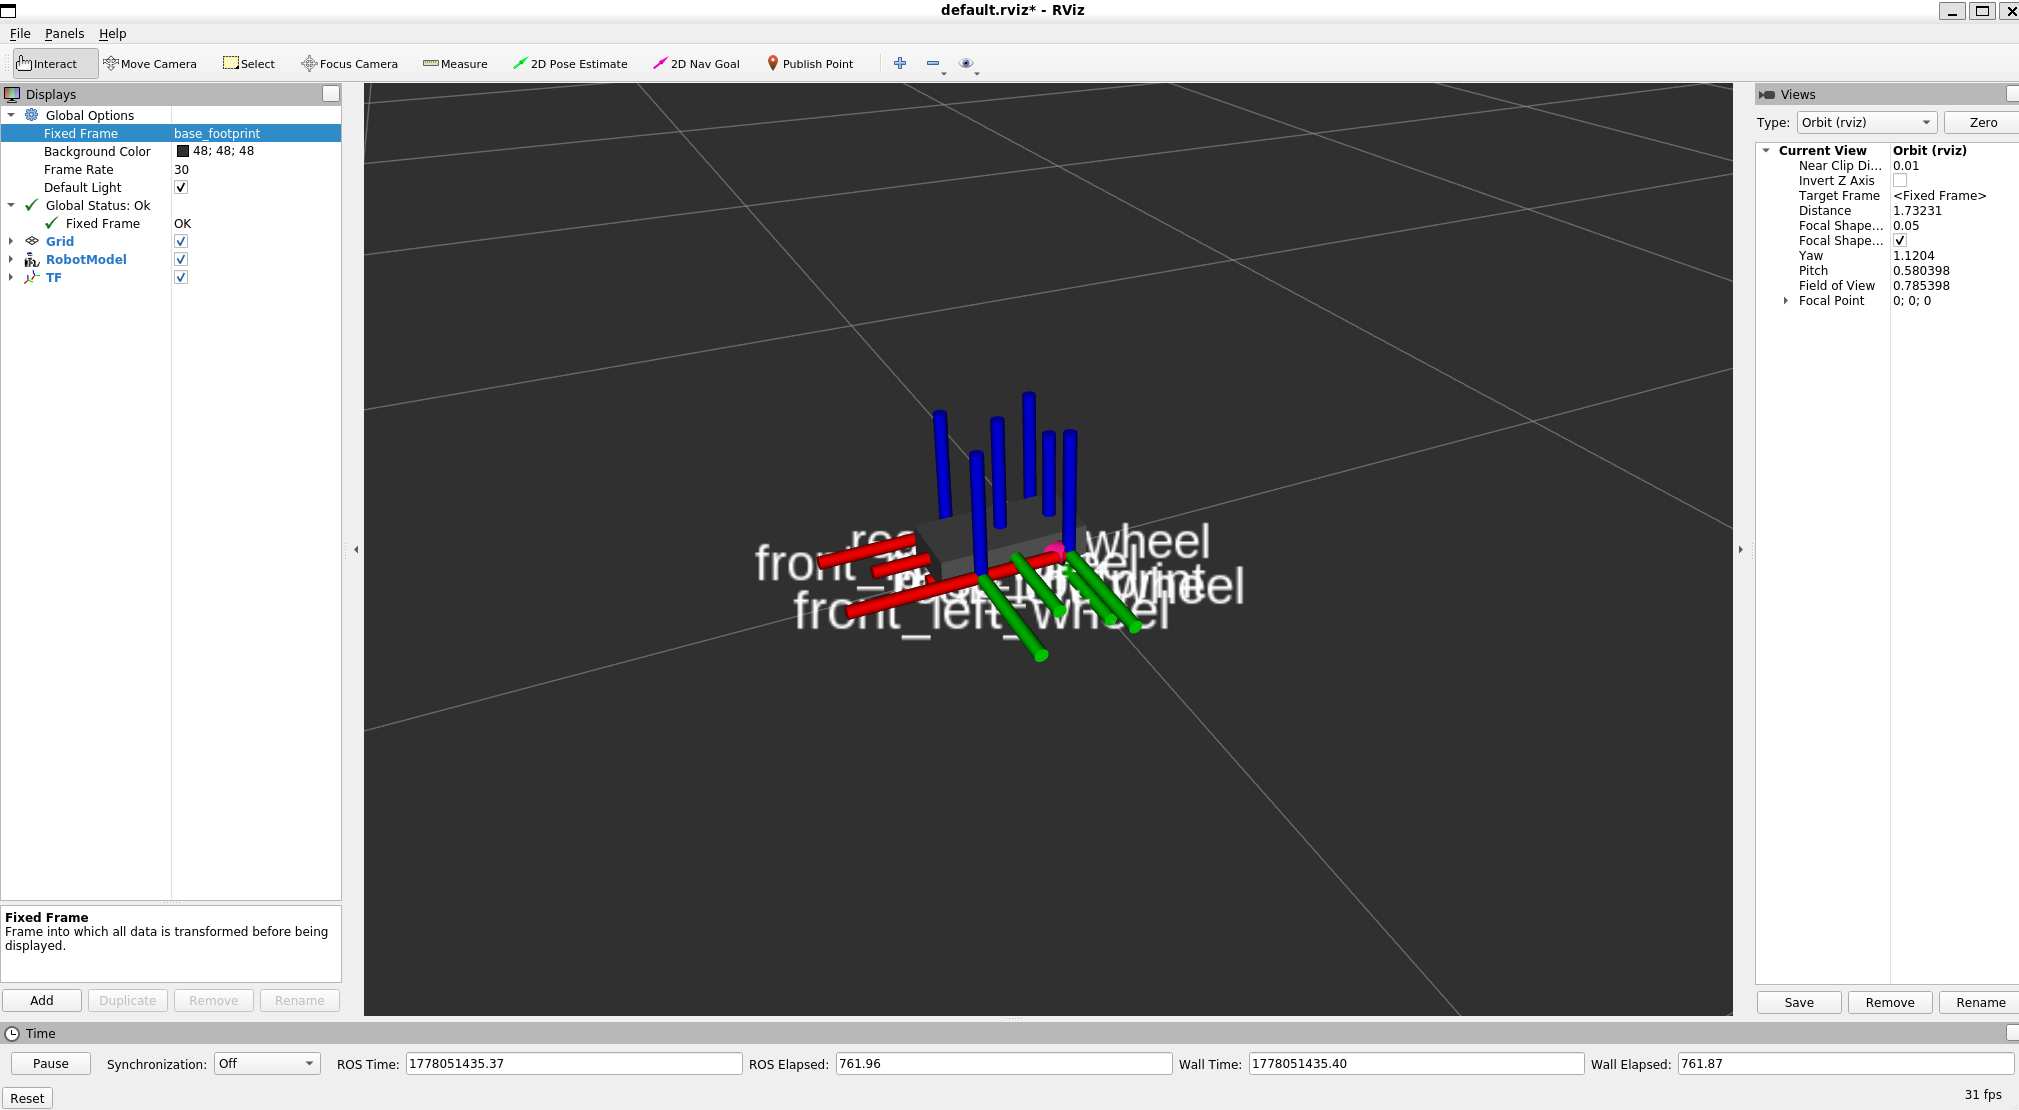
\includegraphics[width=\linewidth]{tf_tree.png}
    \caption{实验中查看到的 TF 树}
  \end{subfigure}
  \caption{仿真实验中的机器人模型和坐标系关系。}
  \label{fig:rviz-tf}
\end{figure}

\subsection{键盘遥控与里程计发布}

在补全 \verb|vehicle_sim.py| 后，仿真节点订阅 \verb|/cmd_vel|，根据线速度和角速度积分得到小车在 \verb|odom| 坐标系下的位置与朝向，并发布 \verb|/odom| 话题和对应 TF。随后使用 \verb|teleop_twist_keyboard.py| 启动键盘控制节点，通过 \verb|u/i/o/j/k/l/m/,/.| 等按键控制平移和旋转，通过 \verb|q/z|、\verb|w/x|、\verb|e/c| 调整最大速度。

运行时，\verb|rostopic info /cmd_vel| 可以看到键盘节点作为发布方，仿真或底盘节点作为订阅方；\verb|rostopic echo /odom| 可以观察到位姿和速度字段随键盘输入持续变化。RViz 中小车模型随控制指令移动，说明速度命令、里程计反馈和 TF 坐标变换三者已经连通。

\subsection{实车悬空测试与落地运动}

实车实验先按照安全要求将小车底盘悬空，连接显示屏、键鼠和电源后启动小车系统，再进入 ROS Noetic 容器启动底盘驱动。悬空测试阶段只观察车轮是否按键盘命令转动，不让小车直接落地运行，可以避免速度方向或控制配置错误导致设备跌落。图 \ref{fig:real-lifted} 截取自实验视频，画面中终端正在运行 \verb|teleop_twist_keyboard|，小车底盘处于悬空调试状态；同时用 \verb|rostopic list|、\verb|rostopic info /cmd_vel| 和 TF 工具检查底盘驱动发布/订阅关系。

\begin{figure}[H]
  \centering
  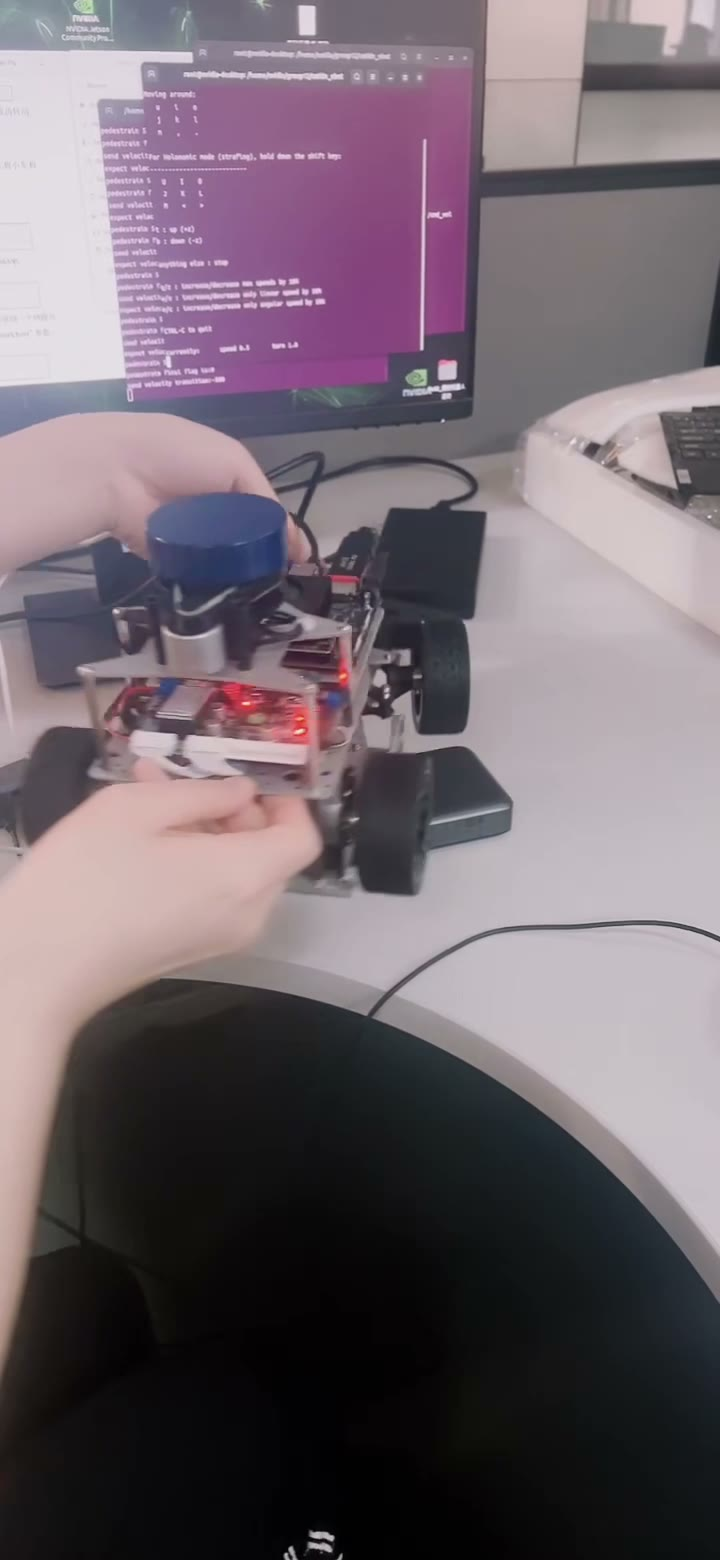
\includegraphics[height=0.34\textheight]{real_car_lifted_test.jpg}
  \caption{实车悬空状态下运行键盘遥控节点并测试车轮响应。}
  \label{fig:real-lifted}
\end{figure}

悬空测试通过后，将小车放到地面继续测试。图 \ref{fig:real-ground} 为第二段视频中截取的运动前后两帧，小车在键盘控制下完成了位置变化，说明 PC 端或小车端发布的 \verb|/cmd_vel| 能够被底盘驱动正确接收并转换成电机控制量。实验过程中，小车运动速度较低，路径附近保持空旷，符合实车测试的基本安全要求。

\begin{figure}[H]
  \centering
  \begin{subfigure}{0.48\linewidth}
    \centering
    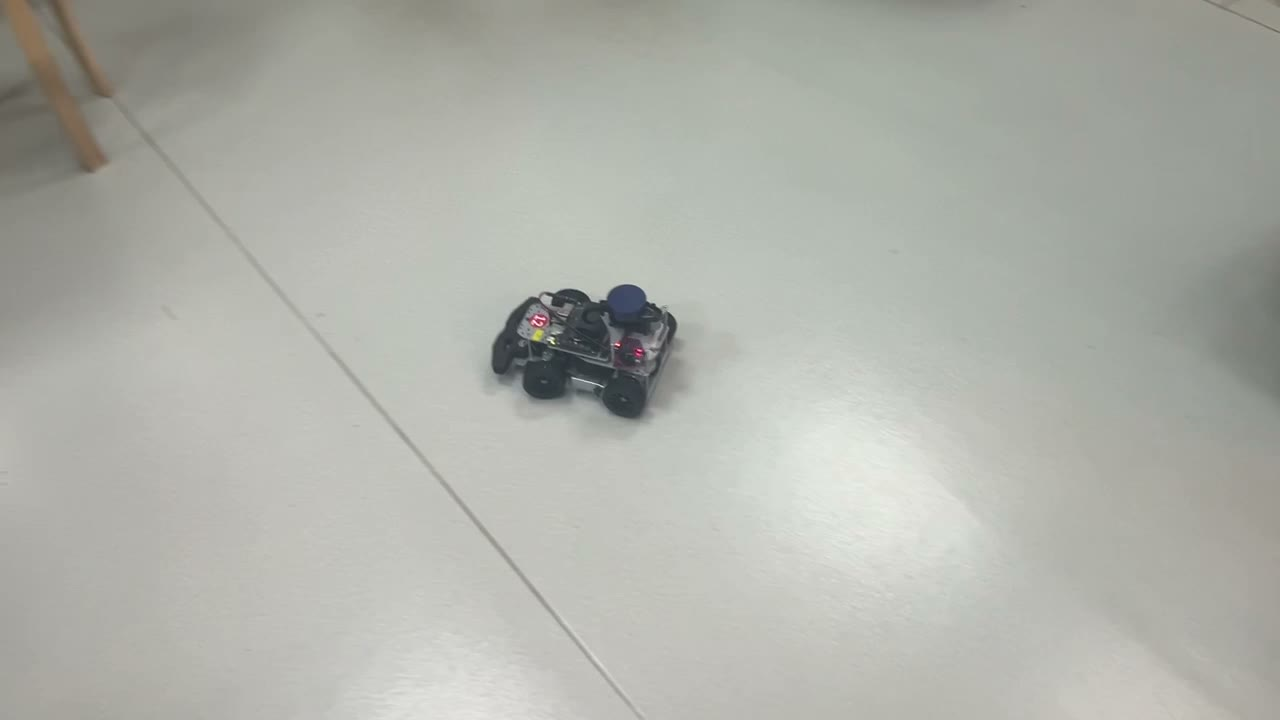
\includegraphics[width=\linewidth]{real_car_ground_start.jpg}
    \caption{落地运动初始位置}
  \end{subfigure}
  \hfill
  \begin{subfigure}{0.48\linewidth}
    \centering
    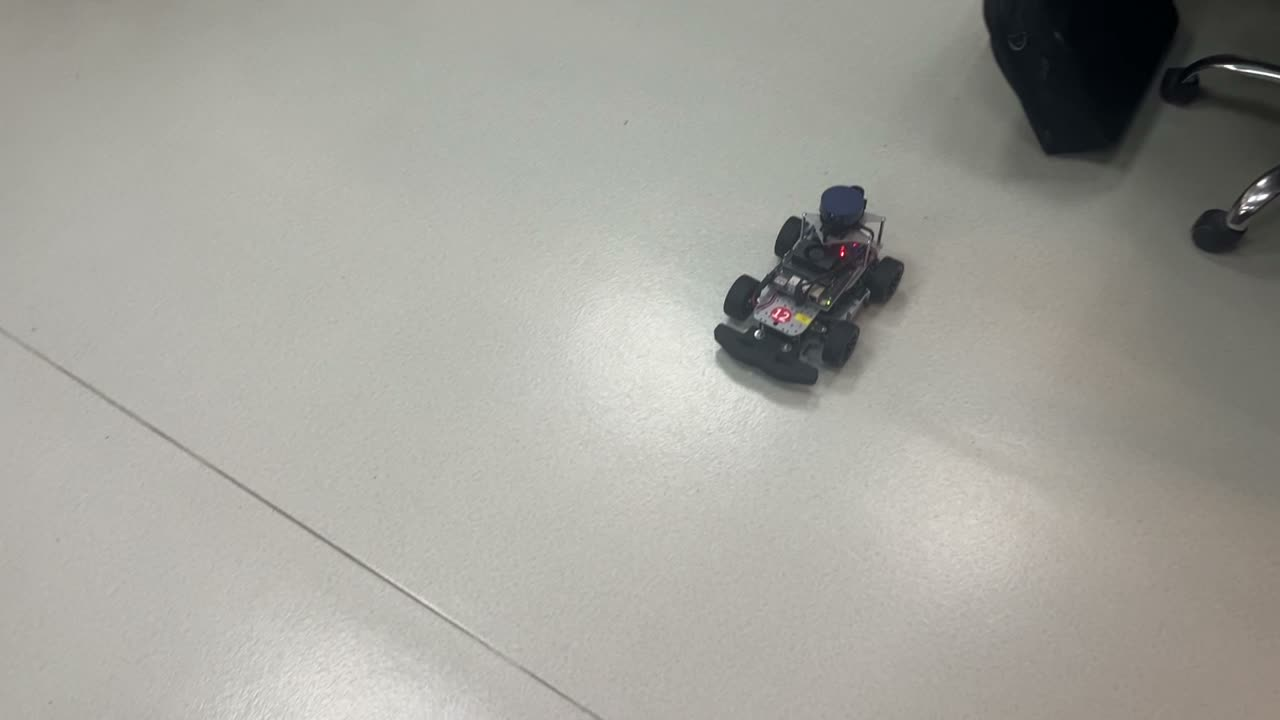
\includegraphics[width=\linewidth]{real_car_ground_motion.jpg}
    \caption{键盘控制后的位置}
  \end{subfigure}
  \caption{实体小车在地面上的键控运动结果。}
  \label{fig:real-ground}
\end{figure}

\section{结论}

本次实验完成了指导书规定的四类任务：配置 ROS 与小车运行环境；在仿真中补全 \verb|vehicle_sim.py|，构建并发布 \verb|odom_frame| 与 \verb|base_frame| 之间的 TF；分别在仿真与实车中查看 TF 树；启动小车底盘并完成远程键盘控制。实验结果说明，URDF 模型可以通过 \verb|robot_description|、\verb|joint_state_publisher| 和 \verb|robot_state_publisher| 在 RViz 中显示，\verb|teleop_twist_keyboard| 发布的 \verb|/cmd_vel| 可以驱动仿真节点或底盘驱动，实车悬空测试和落地运动也验证了底盘控制链路正常。

\section{思考题}

\textbf{\texttt{/odom} 坐标系与 \texttt{/odom} 话题的区别。} \verb|odom| 坐标系是 TF 树中的一个参考坐标系，通常作为里程计定位的父坐标系，用来描述机器人底盘坐标系相对于起始位置的连续运动关系。它的优点是短时间内连续平滑，不会突然跳变；缺点是会随轮速积分产生累计误差。\verb|/odom| 话题则是一个 ROS 数据通道，消息类型通常为 \verb|nav_msgs/Odometry|，其中包含机器人在 \verb|odom| 坐标系下的位姿、速度和协方差信息。简单说，\verb|odom| 是坐标系名称，\verb|/odom| 是发布里程计数据的话题。

\textbf{\texttt{/cmd\_vel} 和 \texttt{/odom} 的发布方、订阅方及关系。} 在仿真和实车中，\verb|/cmd_vel| 通常由键盘遥控、导航规划或上层控制节点发布，由仿真节点或底盘驱动节点订阅；\verb|/odom| 通常由仿真节点或底盘驱动节点发布，由 RViz、导航模块、定位模块等订阅。二者的关系是“控制输入”和“状态反馈”：\verb|/cmd_vel| 表示希望机器人怎样运动，\verb|/odom| 表示机器人根据速度命令和底盘反馈估计出来的实际运动状态。只有同时关注这两个话题，才能判断控制指令是否被正确执行，以及机器人状态是否与预期一致。

\end{document}
